\begin{frame}{Introduction}
	\vfill
	\begin{quotation}
		\centering
		Game theory is the mathematical study of interaction\\
		among independent, self-interested agents.\\
		{\color{colornote}-- Essentials of Game Theory, \cite{leyton2008essentials}}
	\end{quotation}

	\vfill
	\textbf{e.g.} economy and ecology, learning, control, etc. \textcolor{coloraccent}{$\rightsquigarrow$ \emph{cybernetics}.}

	\vspace{-2ex}
	\onslide<2->{
		\begin{center}
			\begin{minipage}{.75\textwidth}
				\begin{block}{}
					\quad \textbf{“Does all this have any practical applications?”} It’s really intriguing because this question is asked in almost exactly the same words wherever I go. [...]

					\quad I ask them, what do you think constitutes a practical application? [...] Roughly speaking, people converge within five to 10 minutes onto two categories of practical applications. \textbf{One is, if you manage to make several million dollars instantly. The other is, if you manage to kill millions of people instantly}. Many people are actually kind of shocked by their own answers.\\
					{\color{colornote}-- Tadashi Tokieda, from \href{https://www.quantamagazine.org/tadashi-tokieda-collects-math-and-physics-surprises-20181127/}{Quanta Magazine}}
				\end{block}
			\end{minipage}
		\end{center}

		\vfill
		\largetext{
		\bfseries
		\hspace{5ex}Game theory shows cooperation is hard...\\
		\hspace{10ex} ...hopefully better math facilities will make it easier!
		}
	}
\end{frame}

\begin{frame}{Introduction}
	\vfill
	Classical game theory: \textbf{normal form} and \textbf{extensive form}

	\begin{center}
		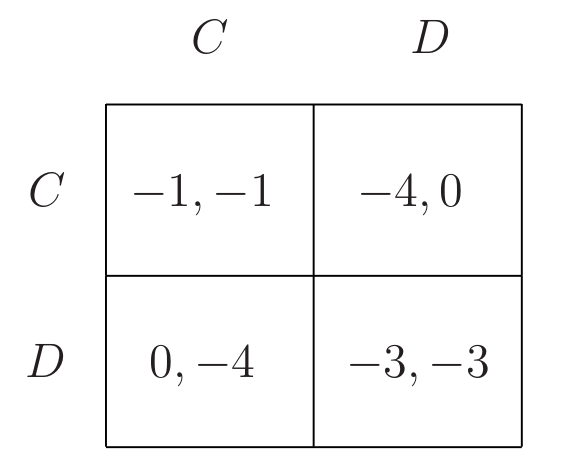
\includegraphics[width=.34\textwidth]{figures/pd_norm.png}
		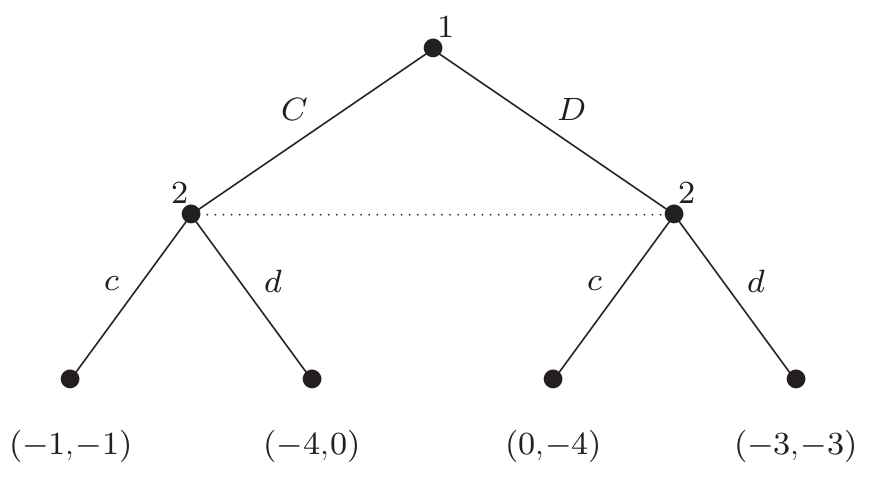
\includegraphics[width=.5\textwidth]{figures/pd_ext.png}
	\end{center}

	\textbf{Drawbacks}:
	\begin{enumerate}
		\item Too little information (NF)... \emph{how is the game actually played?}
		\item Too much information (EF)... \emph{exponential in the number of moves!}
		\item Unclear causal relationships (both).
		\item Most importantly: non-compositional! (\textcolor{coloraccent}{$\rightsquigarrow$ small scale})
	\end{enumerate}
\end{frame}

\begin{frame}{Introduction}
	\textbf{Open games} are a categorical framework for compositional game theory\footnote[frame]{\cite{ghani2018compositional}}:

	\vfill
	\begin{center}
		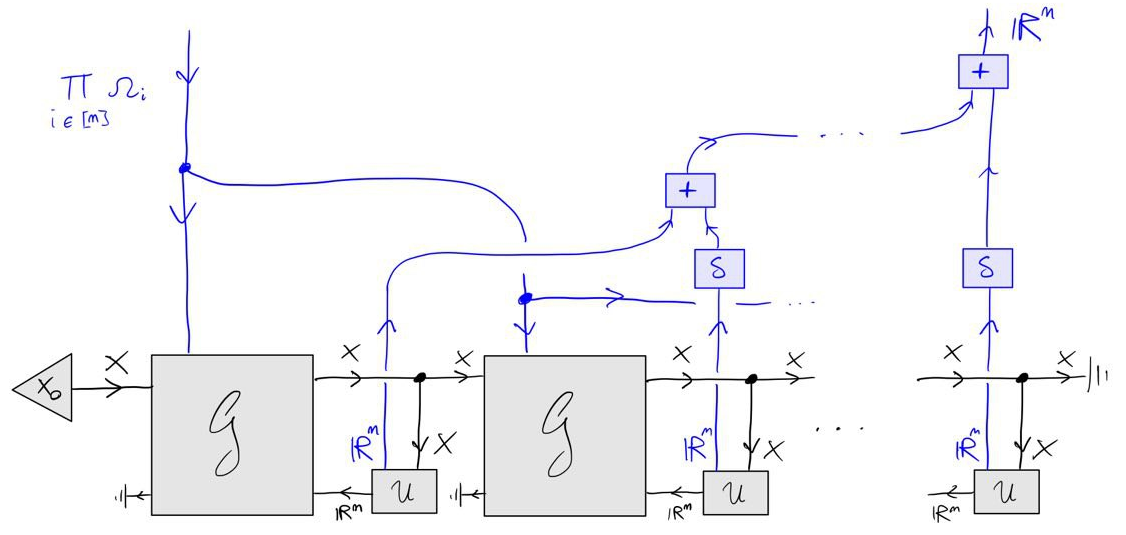
\includegraphics[width=.85\textwidth]{figures/og_ex.png}
	\end{center}

	\vfill
	\textbf{Advantages}:
	\begin{enumerate}
		\item Detailed but not unwieldly... compact notation and true causality
		\item Compositional \& diagrammatic (\textcolor{coloraccent}{$\rightsquigarrow$ large scale}).\\
	\end{enumerate}
\end{frame}

\begin{frame}{Introduction}
	\only<1>{
		Translating normal form games to open games is `trivial'...

		\begin{center}
			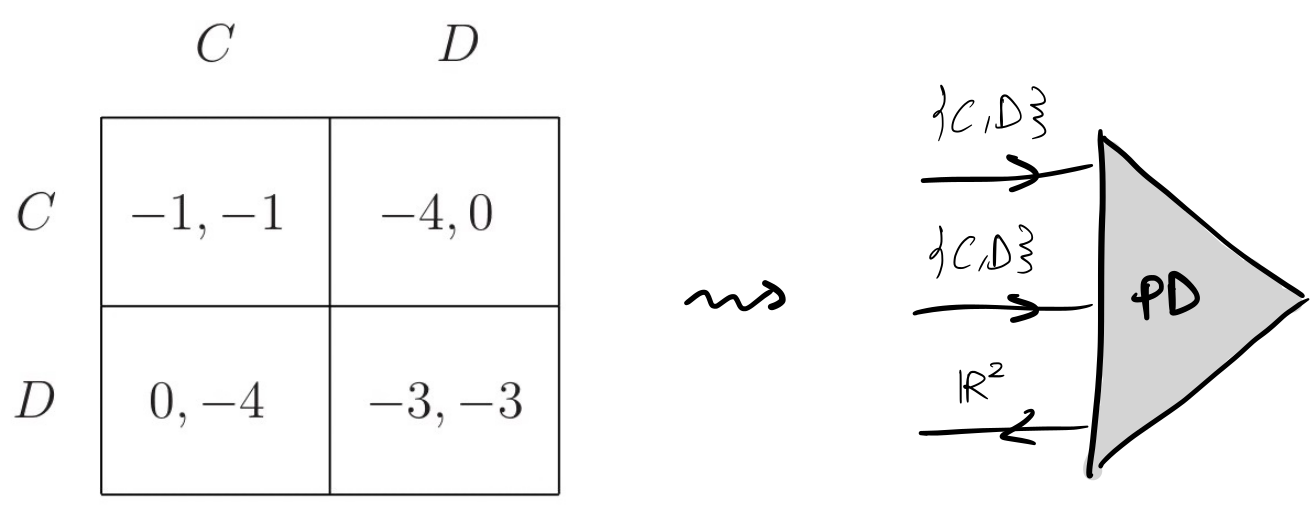
\includegraphics[width=.7\textwidth]{figures/nf_to_og.png}
		\end{center}
	}
	\only<2->{
		Translating extensive form games to open games is non-trivial:
		\begin{enumerate}
			\item We need to seriously consider the problem of agency:
			\begin{enumerate}
				\item How do we represent \textbf{correlated interests} across a game?
				\item How do we represent \textbf{player-dependent observational constraints}?
			\end{enumerate}
			\item We need \textbf{adequate composition operators} to reflect the structure of the game.
		\end{enumerate}

		\vfill
		\onslide<3->{
			To do so, we introduce:

			\begin{enumerate}
				\item \textbf{Open games with agency}, an improved compositional (and conceptual) framework for games,
				drawing from/inspiring `open cybernetic systems'\footnote[frame]{\cite{capucci2021towards}}.
				\item An operator calculus for games, in particular new \textbf{choice operators}.
				%\item \textbf{Inductive data types for EF trees} with (im)perfect information.
			\end{enumerate}
		}
	}
\end{frame}

